\chapter{Method}
We have trained a model to predict emotions, and in order to achieve this we created a dataset with bio metric data for eight emotion categories. We conducted a study where we wanted to elicit emotions in subjects, by having the subjects watch 16 video clips, spanning eight emotion categories.
%We have conducted experiments with the intention of collecting bio data, which we included in a model to predict emotions. This model is supposed to be used as a tool in a video player setting, where we are interested in determining a viewers current emotional state while watching video. Beyond that we are interested in the ability to change the emotional state of a viewer, by introducing video that is supposed to elicit a specific emotion. Subjects will be wearing a skin conductance and heart rate monitor wearable during experiments.

\section{Shimmer3 GSR+ Application} \label{sec:shimmer}
We used Shimmer3 GSR+ \cite{shimmer3} to gather GSR and PPG data. The Shimmer3 GSR+ provides connections and preamplification for one channel of GSR data acquisition as well as capturing a PPG signal. Both the GSR and PPG sensors are secured to the participants fingers, as shown in \cref{pic:shimmer}. The sensors are secured using velcro straps, which can be a sourced of imprecision if the sensors are secured improperly.

\begin{figure}[H]
    \centering
    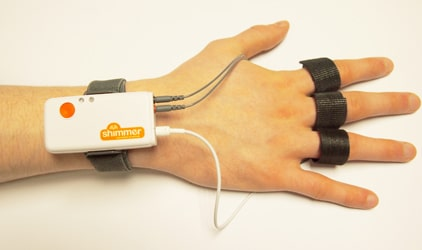
\includegraphics[width=8cm]{pictures/shimmer.jpg}
    \caption{The Shimmer3 GSR+ being worn}
    \label{pic:shimmer}
\end{figure}

\subsection{Application for reading GSR and PPG data}
Data from the Shimmer unit is collected by with an application developed by Cinematronic for the specific purpose of recording data while playing a video. The application has been slightly modified to be a better fit for our specific use case, such as allowing for the collection of PPG data. The application window can be seen on \cref{pic:test-env}.

\begin{figure}[H]
    \centering
    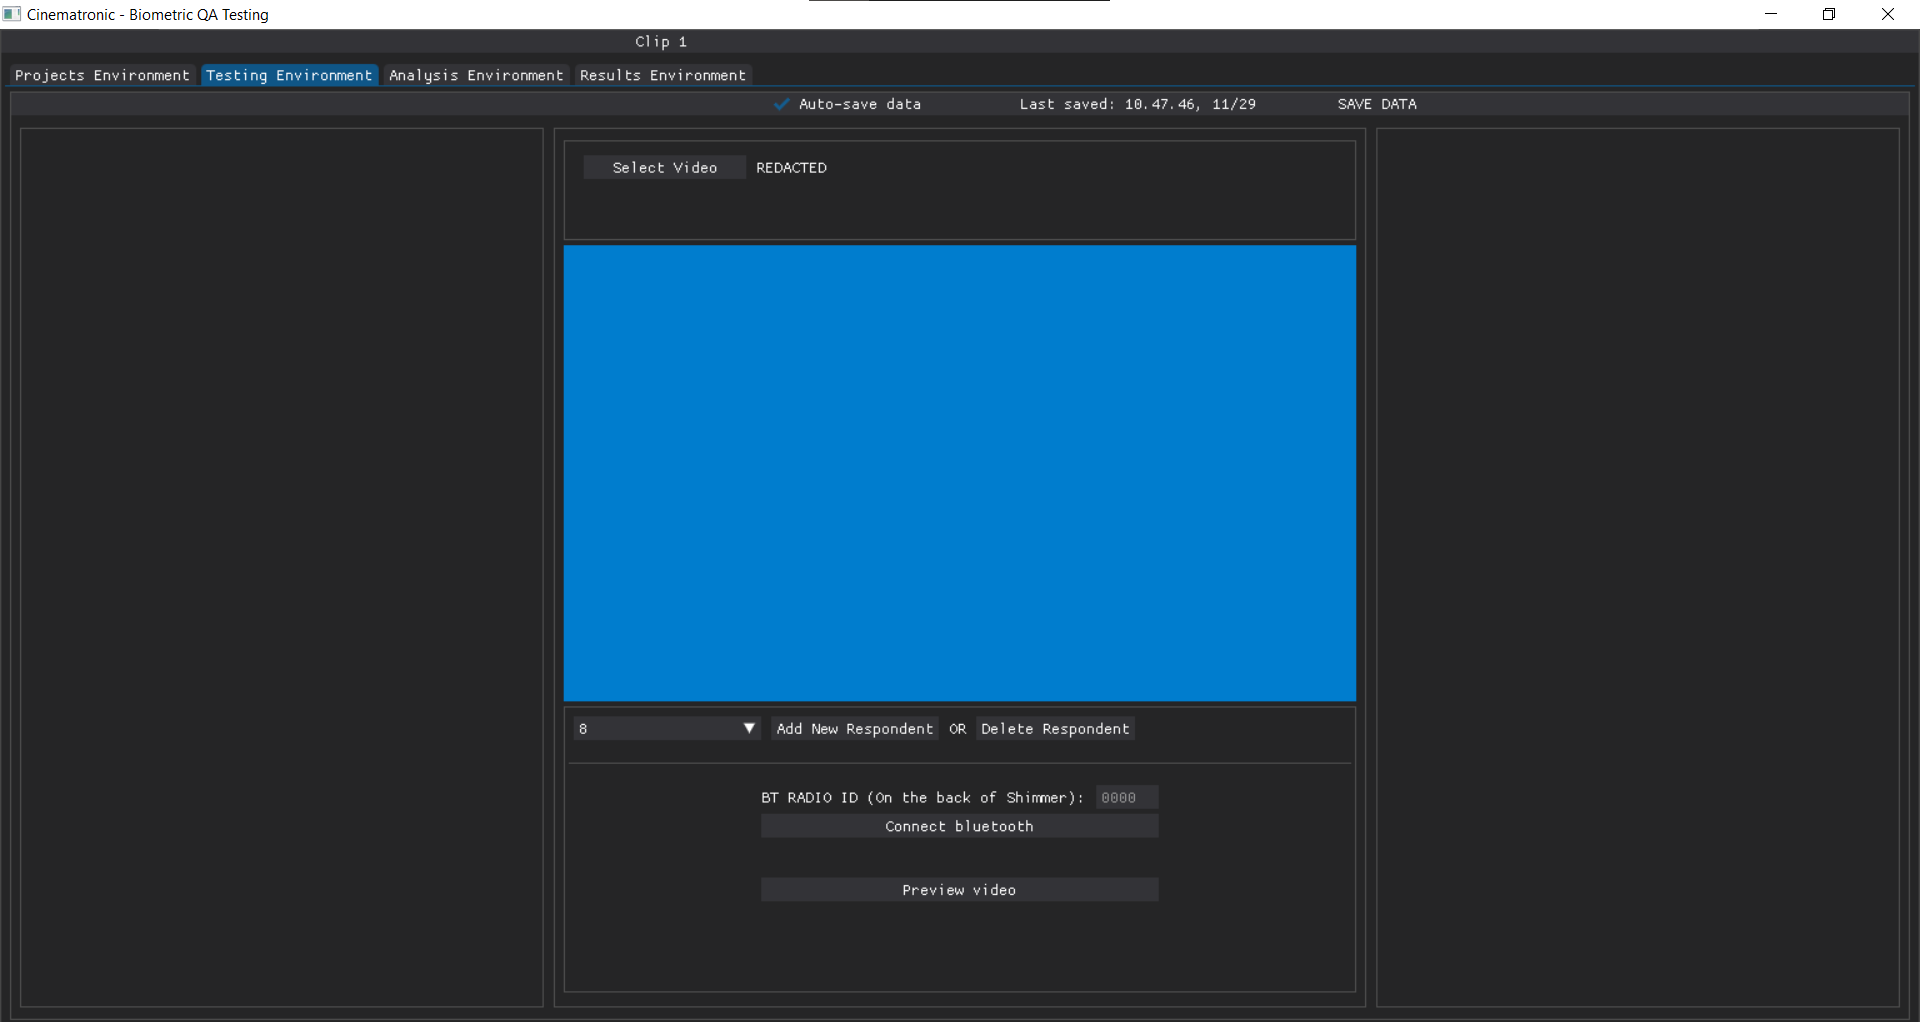
\includegraphics[width=15cm]{pictures/Testing_env.png}
    \caption{The testing screen of the application}
    \label{pic:test-env}
\end{figure}

\noindent An example of how the data is formatted once a participant is done watching a video can be seen on \cref{pic:anal-env}. Here the orange graph represents the PPG data, and the blue represents the GSR data.

\begin{figure}[H]
    \centering
    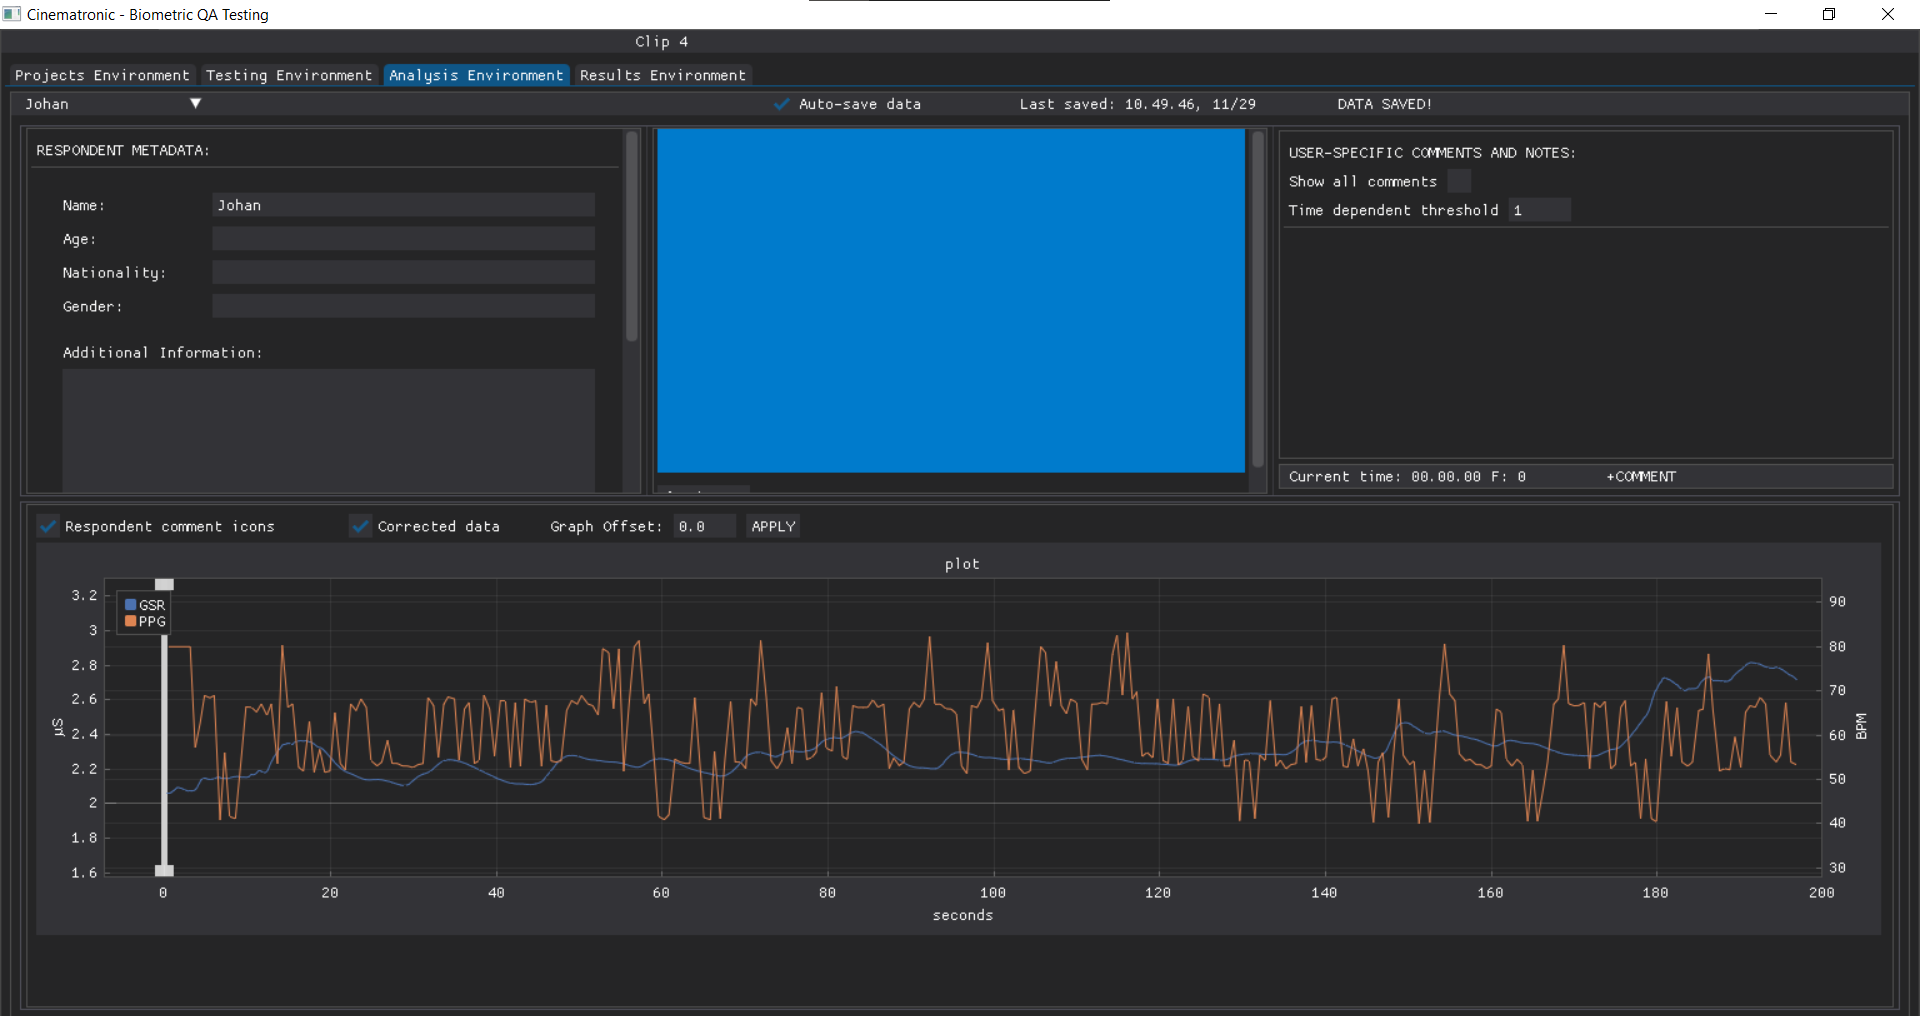
\includegraphics[width=15cm]{pictures/Analysis_env.png}
    \caption{The analysis screen of the application}
    \label{pic:anal-env}
\end{figure}


\section{Selecting Emotions}\label{sec:selectingEmotion}
Based on related work presented in \Cref{cap:relatedWork} we have decided on the following eight emotional states. These eight emotions are derived from Ekmans six core motions which all overlap with Izards ten. We mapped the eight emotions to the valence/arousal space according to Russel. We chose neutral and relaxed to fill out the spaces in the valence/arousal model and because these have been used in other studies of eliciting emotions.
\begin{itemize}
    \item Anger
    \item Fear
    \item Disgust
    \item Sadness
    \item Joy
    \item Surprise
    \item Relaxed
    \item Neutral
\end{itemize}
These are mapped to the valence-arousal space according to \cref{fig:VAinit}. The emotions shown on the figure would not be as ordered as displayed. In reality, the emotions would have some overlap, but in order to make a definite decision, a clear cut approximation has been made.

\begin{figure}[H]
    \centering
    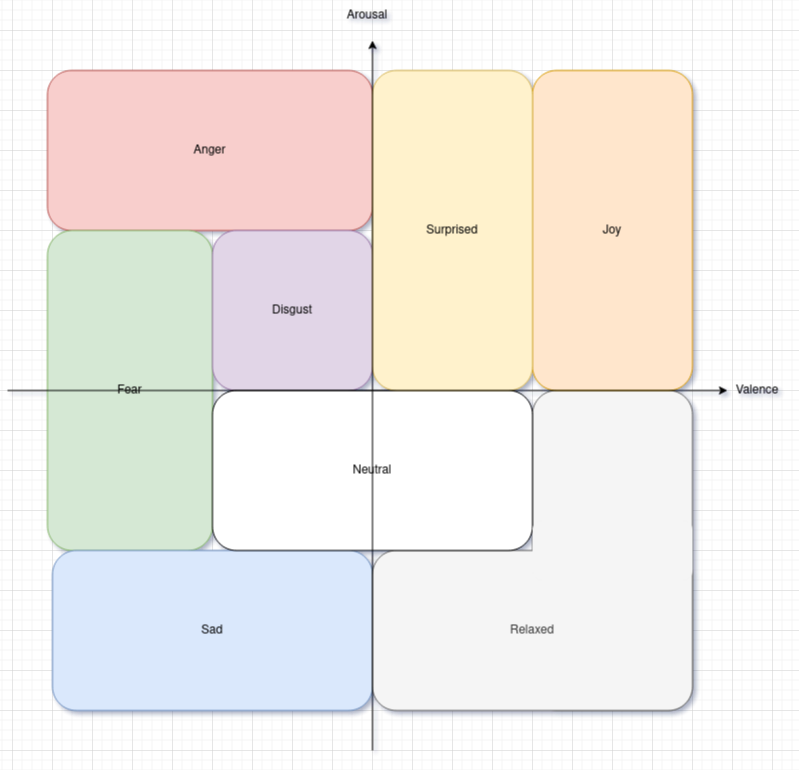
\includegraphics[width=\textwidth]{figures/va16model.png}
    \caption{Initial valence-arousal model}
    \label{fig:VAinit}
\end{figure}

\section{Eliciting Emotions}
In order for us to elicit emotions for subjects in an experimental setting we decided to show subjects video clips, each labeled with one of the emotions outlined in \cref{sec:selectingEmotion}. We decided on this setup because our end goal is generating video in conjunction with bio metric data, thus gathering bio metric data from video viewing made sense.
\\ \\
\subsection{Criteria for Choosing Videos from Emotion Eliciting Datasets}
The value of each dataset is weighted according to three criteria, which are evaluated in order to ensure that the dataset is capable of evoking the desired emotions.
\\ \\
\textbf{First criterion}\\
The dataset is required to use videos as the source of media to gather emotions. This criterion was included as we wish to combine the use of video and sound in order to evoke emotions.
\\ \\
\textbf{Second criterion}\\
The dataset is required to have some kind of evaluation or ranking of the videos. Such a criterion will ensure transparency as to how well a given video was able to evoke the desired emotion. It also stands to reason that certain videos are better at eliciting certain emotions than others, so a way to compare the videos is desirable.  
\\ \\
\textbf{Third criterion}\\
The dataset is required to have at least 5 minutes of media data for each emotion. This criterion was included by us, as less than this amount of data will not be feasible to collect sensor data.
\\ \\
We searched google scholar with the keywords "eliciting emotions", "eliciting emotions movie" and "eliciting emotions video". This search yielded a large amount of dataset, but many of them did not fulfill our criteria, and others were not accessible without requesting access, which could take up to a month. We narrowed it down to five datasets, which was explored further as they had all been widely used in similar research, yielding good results. The datasets are outlined below, explaining their use cases and how they fit with our criteria.
\\ \\
\textbf{FilmStim} is a video database containing 70 labeled clips from known movies \cite{FilmStim}. The dataset is made with the explicit purpose of making a freely available dataset that would be as adaptable as possible to a wide array of research questions. The labels contains six emotions: anger, fear, sadness, disgust, amusement, tenderness and additionally neutral, with clips ranging from one to seven minutes in length. The emotional responses elicited by these clips are validated by 364 participants, each viewing 10 clips. The emotional states of the participants where assessed by a emotional arousal scale, the Differential Emotions Scale and  the Positive and Negative Affect Schedule. All are self-reported by the participants. \newline
Although the original dataset was compiled for french language, it has since been updated with English versions where available, which is 52 out of the 70 clips. This dataset is overall very usable for this project, most of the English movie clips can be used and might even be too much for this project.
\\ \\
\textbf{FilmClips} , an attempt is made to construct a modern dataset of film clips that is able to evoke basic and complex emotions \cite{FilmClips}. A total of 14 emotions are measured, using the arousal and valance model. The dataset is constructed by performing two separate studies, where participants watched film clips and rated the clips according to the degree of emotion that they evoked. The paper was able to discretely elicit 11 different emotions and consists of a total of 50 film clips. Relating this to the criteria, both are fulfilled as it maps to 11 different emotions and consists of a range of videos for each emotion.
\\ \\
\textbf{The CASE: Continuous affect annotations and physiological signals} for emotion analysis dataset features 30 participants who watched eight videos of 2-3 minutes, two for each of the four emotions: amusing, boring, relaxing and scary. That is one emotion for each valence/arousal quadrant. The videos were selected based on previous datasets and includes movie clips, documentaries and nature videos. To avoid the carried bias from changing videos, each participant watched the videos in random order while there was a two minute span of blue screen between each video. What is special about this dataset is that the participants log their own emotional state to a valence/arousal graph in real time using a joystick. \cite{CaseData}
This dataset is somewhat usable, while only four emotions is however in the low-end and boring and relaxing seem somewhat similar.
\\ \\
\textbf{DEAP: A Database for Emotion Analysis} is a widely used multimodal dataset for the analysis of human affective state. It was originally created for the purpose of creating an adaptive music video recommendation system. For this purpose, the dataset consists of 120 one-minute excerpts from music videos, that each fit into one of 16 emotional states. Each clip is rated by 14-16 participants based on arousal, valence, and dominance. However, the range of 16 emotional states are far too specific for use in this particular study, so the dataset would need to be generalized in some way to only cover the relevant emotional states, mentioned in \cref{sec:emotionalModel}.
Furthermore, the media type of the dataset being music videos adds an additional emotional response trigger through sound elements, which is not a particularly good fit for this specific use case. The dataset is not publicly available, so it is necessary to apply to gain access, which is not guaranteed. \cite{DEAP} \newline
This dataset does not exactly fit the use case of this study, and is not publicly available. However, the described method for identifying relevant videos could be useful. 
\\ \\
\textbf{Chen H et al.} describes the process of selecting a collection of professional and amateur videos eliciting five basic emotions: happiness, fear, disgust, anger and sadness. The dataset primarily consists of movie trailers for the professional videos and YouTube videos for the amateur videos. All videos are less than one minute.
The participants were split into three groups, with different nationalities, to ensure that the videos could elicit emotions, even though they could not understand the language. 20 professional and 20 amateur videos were chosen, and 30 participants were given the task of identifying and rating the emotions they felt. The dataset is the 40 videos with accompanying rating data. \cite{CHEN2021106662}.
This dataset is somewhat usable in that it aims to elicit five strong and different emotions. Unfortunately some videos are very short, down to 5 seconds. However, there are many videos for each emotion, allowing us to choose the ones that makes most sense or put some of the short videos together in sequence.

\subsubsection{Our Selection}
None of the above datasets cover all the emotional states we want to cover. Because of this we will use the videos from those datasets, when publicly available, that relate to the emotions we aim for. Some emotions have many related videos. For these we will choose two videos for each emotion, choosing those best shown to elicit the relevant emotion, based on the datasets own evaluation. \Cref{tab:videos} show which videos for each dataset are relevant for the chosen emotions and which we choose for our dataset.
%Based on the datasets we have just presented we will now explain how we construct the dataset that we will use for our experiments. 

\begin{table}[]
    \centering
    \begin{tabular}{|c|c|c|c|c|c|c|}
        %Happy
        \hline
        ID & Origin & Emotion & Length (m:s) & Evaluation & Source\\ \hline
        1 & The Pursuit of Happyness (subway) & Sad & 4:20 & 7.6  & FilmClips \cite{FilmClips} \\ \hline
        2 & I Am Sam & Sad & 2:16 & 7.9  & FilmClips \cite{FilmClips}\\ \hline
        3 & The Conjuring & Fear & 3:04 & 7.3  & FilmClips \cite{FilmClips}  \\ \hline
        4 & Insidious & Fear & 3:08 & 6.95  & FilmClips \cite{FilmClips} \\ \hline
        5 & Ex Machina & Neutral & 0:59 & 6.9  & FilmClips \cite{FilmClips} \\ \hline
        6 & Rudderless (buisness meeting) & Neutral & 0:43 & 6.8  & FilmClips \cite{FilmClips} \\ \hline
        7 & Soul Surfer (homeless girl) & Joy & 2:31 & 7.6  & FilmClips \cite{FilmClips} \\ \hline
          %Coach Carter (honoring coach) & Joy & 0:43 & 6.4  & FilmClips \cite{FilmClips} & Yes \\ \hline
          %Coach Carter (winning basket) & Joy & 1:33 & 7.3  & FilmClips \cite{FilmClips} & Yes \\ \hline
        8 & Forrest Gump (reunion) & Joy & 1:12 & 7.5  & FilmClips \cite{FilmClips} \\ \hline
        9 & Slumdog Millionaire (blinded) & Disgust & 1:46 & 8.3  & FilmClips \cite{FilmClips} \\ \hline
        10 &  Trainspotting [2] & Disgust & 1:14 & 4.07  & FilmStim \cite{FilmStim} \\ \hline
        11 & Sleepers & Anger & 2:34 & 2.72  & FilmStim \cite{FilmStim}  \\ \hline
        12 & American History X & Anger & 1:31 & 1.94  & FilmStim \cite{FilmStim} \\ \hline
        13 & One day & Surprise & 0:37 & 7.5 & FilmClips \cite{FilmClips}\\ \hline
        14 & Deep Blue Sea & Surprise & 2:14 & 7.7 & FilmClips \cite{FilmClips} \\ \hline
        15 & Relaxing Piano Music - Nature Scenes & Relaxed & 2:10 & N/A & CASE \cite{CaseData}  \\ \hline
        16 & Relaxing Sunset To Nightfall Relaxation Meditation & Relaxed & 2:10 & N/A & CASE \cite{CaseData} \\ \hline
    \end{tabular}
    \caption{Chosen videos. Total time is 32 minutes and 29 seconds.}
    \label{tab:videos}
\end{table}

\section{Experimental Setup}
In this study, we use the dataset shown in \cref{tab:videos} to collect GSR and PPG data within the different arousal and valence levels that was chosen to represent the emotional states. The aim is to collect GSR and PPG data for a range of participants, all of which has an emotion-label associated with it. This emotion-label falls within the combination of the four-level arousal and valence model.
\subsection{Participants}
XX volunteers from the university community participated in the study. There was made no distinct choice in age, nationality, race, gender, etc. of the participants, as none of these factors have any relevant impact on the data collected.    
\subsection{Data collection}
All GSR and PPG data was collected using the Shimmer3 GSR+, as explained in \Cref{sec:shimmer}, while wearing a noise-cancelling headset to eliminate any distractions.
Furthermore, all data was collected in the same room to ensure as little variability in the environment as possible, as variance in temperature and lighting can have an impact on the participants biological reaction.
\subsection{Task and procedure}
The study progressed in a simple manner. Each participant was placed in the room, and made to watch the 16 videos outlined in \cref{tab:videos}, in a random order. This was done to ensure the data we collected was not situational, as the participants reaction could be somewhat impacted by the previous video. In this regard, each video also started with ten seconds of blue screen, to allow the participant to calm down before the next video begins.\\
After each video, the participant was asked to evaluate the intensity they felt for each emotion using a five-point Likert scale. We did this so the participant could provide their own label to how they felt watching the clip, and to see if they diverted from the expected emotion of the clip. Repeating this process for each clip ended up taking about an hour for each participant.
\subsection{Results}
The result of this study is a dataset of labeled GSR and PPG data that can be used to construct the emotion detection model.